% Options for packages loaded elsewhere
\PassOptionsToPackage{unicode}{hyperref}
\PassOptionsToPackage{hyphens}{url}
%
\documentclass[a4paper
]{article}
\author{}
\date{}

\usepackage[a4paper, margin={0.5in, 0.75in}]{geometry}


\usepackage{amsmath,amssymb}
\usepackage{lmodern}
\usepackage{iftex}
\ifPDFTeX
  \usepackage[T1]{fontenc}
  \usepackage[utf8]{inputenc}
  \usepackage{textcomp} % provide euro and other symbols
\else % if luatex or xetex
  \usepackage{unicode-math}
  \defaultfontfeatures{Scale=MatchLowercase}
  \defaultfontfeatures[\rmfamily]{Ligatures=TeX,Scale=1}
\fi
% Use upquote if available, for straight quotes in verbatim environments
\IfFileExists{upquote.sty}{\usepackage{upquote}}{}
\IfFileExists{microtype.sty}{% use microtype if available
  \usepackage[]{microtype}
  \UseMicrotypeSet[protrusion]{basicmath} % disable protrusion for tt fonts
}{}
\makeatletter
\@ifundefined{KOMAClassName}{% if non-KOMA class
  \IfFileExists{parskip.sty}{%
    \usepackage{parskip}
  }{% else
    \setlength{\parindent}{0pt}
    \setlength{\parskip}{6pt plus 2pt minus 1pt}}
}{% if KOMA class
  \KOMAoptions{parskip=half}}
\makeatother
\usepackage[]{xcolor}
\IfFileExists{xurl.sty}{\usepackage{xurl}}{} % add URL line breaks if available
\IfFileExists{bookmark.sty}{\usepackage{bookmark}}{\usepackage{hyperref}}
\hypersetup{
  colorlinks,
  pdfcreator={LaTeX via pandoc}}
\urlstyle{same} % disable monospaced font for URLs
\usepackage{color}
\usepackage{fancyvrb}
\newcommand{\VerbBar}{|}
\newcommand{\VERB}{\Verb[commandchars=\\\{\}]}
\DefineVerbatimEnvironment{Highlighting}{Verbatim}{commandchars=\\\{\}}
% Add ',fontsize=\small' for more characters per line
\newenvironment{Shaded}{}{}
\newcommand{\AlertTok}[1]{\textcolor[rgb]{1.00,0.00,0.00}{\textbf{#1}}}
\newcommand{\AnnotationTok}[1]{\textcolor[rgb]{0.38,0.63,0.69}{\textbf{\textit{#1}}}}
\newcommand{\AttributeTok}[1]{\textcolor[rgb]{0.49,0.56,0.16}{#1}}
\newcommand{\BaseNTok}[1]{\textcolor[rgb]{0.25,0.63,0.44}{#1}}
\newcommand{\BuiltInTok}[1]{#1}
\newcommand{\CharTok}[1]{\textcolor[rgb]{0.25,0.44,0.63}{#1}}
\newcommand{\CommentTok}[1]{\textcolor[rgb]{0.38,0.63,0.69}{\textit{#1}}}
\newcommand{\CommentVarTok}[1]{\textcolor[rgb]{0.38,0.63,0.69}{\textbf{\textit{#1}}}}
\newcommand{\ConstantTok}[1]{\textcolor[rgb]{0.53,0.00,0.00}{#1}}
\newcommand{\ControlFlowTok}[1]{\textcolor[rgb]{0.00,0.44,0.13}{\textbf{#1}}}
\newcommand{\DataTypeTok}[1]{\textcolor[rgb]{0.56,0.13,0.00}{#1}}
\newcommand{\DecValTok}[1]{\textcolor[rgb]{0.25,0.63,0.44}{#1}}
\newcommand{\DocumentationTok}[1]{\textcolor[rgb]{0.73,0.13,0.13}{\textit{#1}}}
\newcommand{\ErrorTok}[1]{\textcolor[rgb]{1.00,0.00,0.00}{\textbf{#1}}}
\newcommand{\ExtensionTok}[1]{#1}
\newcommand{\FloatTok}[1]{\textcolor[rgb]{0.25,0.63,0.44}{#1}}
\newcommand{\FunctionTok}[1]{\textcolor[rgb]{0.02,0.16,0.49}{#1}}
\newcommand{\ImportTok}[1]{#1}
\newcommand{\InformationTok}[1]{\textcolor[rgb]{0.38,0.63,0.69}{\textbf{\textit{#1}}}}
\newcommand{\KeywordTok}[1]{\textcolor[rgb]{0.00,0.44,0.13}{\textbf{#1}}}
\newcommand{\NormalTok}[1]{#1}
\newcommand{\OperatorTok}[1]{\textcolor[rgb]{0.40,0.40,0.40}{#1}}
\newcommand{\OtherTok}[1]{\textcolor[rgb]{0.00,0.44,0.13}{#1}}
\newcommand{\PreprocessorTok}[1]{\textcolor[rgb]{0.74,0.48,0.00}{#1}}
\newcommand{\RegionMarkerTok}[1]{#1}
\newcommand{\SpecialCharTok}[1]{\textcolor[rgb]{0.25,0.44,0.63}{#1}}
\newcommand{\SpecialStringTok}[1]{\textcolor[rgb]{0.73,0.40,0.53}{#1}}
\newcommand{\StringTok}[1]{\textcolor[rgb]{0.25,0.44,0.63}{#1}}
\newcommand{\VariableTok}[1]{\textcolor[rgb]{0.10,0.09,0.49}{#1}}
\newcommand{\VerbatimStringTok}[1]{\textcolor[rgb]{0.25,0.44,0.63}{#1}}
\newcommand{\WarningTok}[1]{\textcolor[rgb]{0.38,0.63,0.69}{\textbf{\textit{#1}}}}
\usepackage{longtable,booktabs,array}
\usepackage{calc} % for calculating minipage widths
% Correct order of tables after \paragraph or \subparagraph
\usepackage{etoolbox}
\makeatletter
\patchcmd\longtable{\par}{\if@noskipsec\mbox{}\fi\par}{}{}
\makeatother
% Allow footnotes in longtable head/foot
\IfFileExists{footnotehyper.sty}{\usepackage{footnotehyper}}{\usepackage{footnote}}
\makesavenoteenv{longtable}
\usepackage{graphicx}
\makeatletter
\def\maxwidth{\ifdim\Gin@nat@width>\linewidth\linewidth\else\Gin@nat@width\fi}
\def\maxheight{\ifdim\Gin@nat@height>\textheight\textheight\else\Gin@nat@height\fi}
\makeatother
% Scale images if necessary, so that they will not overflow the page
% margins by default, and it is still possible to overwrite the defaults
% using explicit options in \includegraphics[width, height, ...]{}
\setkeys{Gin}{width=\maxwidth,height=\maxheight,keepaspectratio}
% Set default figure placement to htbp
\makeatletter
\def\fps@figure{htbp}
\makeatother
\setlength{\emergencystretch}{3em} % prevent overfull lines
\providecommand{\tightlist}{%
  \setlength{\itemsep}{0pt}\setlength{\parskip}{0pt}}
\setcounter{secnumdepth}{-\maxdimen} % remove section numbering
\ifLuaTeX
  \usepackage{selnolig}  % disable illegal ligatures
\fi


% -------fady-------
\usepackage{float}
\usepackage{listings}
% Syntax highlighting style:
\definecolor{codegreen}{rgb}{0,0.6,0}
\definecolor{codegray}{rgb}{0.5,0.5,0.5}
\definecolor{codepurple}{rgb}{0.58,0,0.82}
\definecolor{backcolour}{rgb}{0.95,0.95,0.92}

\lstdefinestyle{mystyle}{
  backgroundcolor=\color{backcolour},   
  commentstyle=\color{codegreen},
  keywordstyle=\color{magenta},
  numberstyle=\tiny\color{codegray},
  stringstyle=\color{codepurple},
  basicstyle=\ttfamily\small,
  breakatwhitespace=false,         
  breaklines=true,                 
  captionpos=b,                    
  keepspaces=true,                 
  numbers=left,                    
  numbersep=5pt,                  
  showspaces=false,                
  showstringspaces=false,
  showtabs=false,                  
  tabsize=2
}


\lstset{style=mystyle}

%-------------------------

% \lstset{
% frameround=fttt,
% language=SQL,
% numbers=left,
% breaklines=true,
% keywordstyle=\color{blue}\bfseries, 
% basicstyle=\ttfamily\color{red},
% numberstyle=\color{black}
% }

\usepackage{titling}
\title{Operationalizing an AWS ML Project}
\author{
  Fady Morris Ebeid
  \thanks{Email: \href{mailto:fadymorris86@gmail.com}{fadymorris86@gmail.com}}
}
\date{January 20, 2022}



\begin{document}
\pagenumbering{roman}
\pretitle{%from package titling
  \begin{center}
    \LARGE
    
\includegraphics[width=0.75\textwidth]{../../../img/udacity-logo}\\[\bigskipamount]
  }


{
\makeatletter
\addtocounter{footnote}{1} % to get dagger instead of star
\renewcommand\thefootnote{\@fnsymbol\c@footnote}%
\makeatother
\maketitle
}
\newpage
\tableofcontents

\newpage
\pagenumbering{arabic}

\hypertarget{project-directory-structure}{%
\section{Project Directory
Structure}\label{project-directory-structure}}


\begin{lstlisting}[caption=Project Directory Structure]
├── doc
│   └── writeup.pdf                           # Project writeup document.
├── ec2train1.py                              # Python training script used inside EC2 instance.
├── hpo.py                                    # Hyperparameter tuning and model training script.
├── infernce2.py                              # Endpoint inference script (entry point)
├── lambda-deployment-testing-security.ipynb       # Custom notebook to deploy and test lambda function.
├── lamdafunction.py                               # Lambda function entry point (modified to include the endpoint name)
├── README.md
├── screenshots                               # Project screenshots.
├── train_and_deploy-solution.html            # HTML export of the solution notebook
└── train_and_deploy-solution.ipynb           # Solution notebook
\end{lstlisting}
% \end{verbatim}

\newpage
\hypertarget{step-1-initial-setup-training-and-deployment}{%
\section{Step 1: Initial setup, training and
deployment}\label{step-1-initial-setup-training-and-deployment}}

\hypertarget{initial-setup}{%
\subsection{Initial Setup}\label{initial-setup}}

First, we start by creating a sagemaker notebook instance. In this case
I cose \texttt{ml.t2.medium} instance it is the most economic instance
type in sagemaker. and we don't need powerful processing power or large
RAM. This instance will be used for just running notebook code and will
not be used for model training or inference.

A screenshot of the notebook instance:

\begin{figure}[H]
\centering
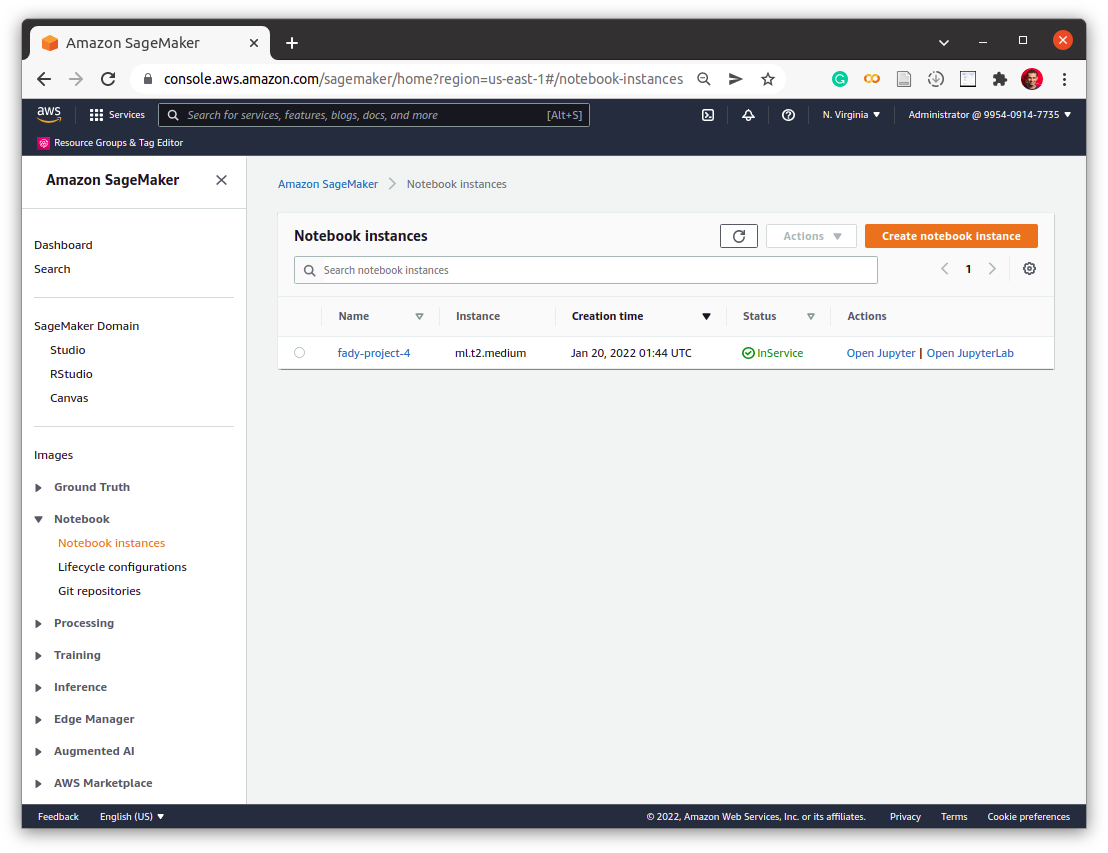
\includegraphics[]{../screenshots/01-a_sagemaker-notebook-instance.png}
%\caption{Notebook Instance}
\end{figure}

Then upload code archive
\href{https://video.udacity-data.com/topher/2021/September/613fd77f_starter/starter.zip}{\texttt{starter.zip}}
to the notebook instance to run the experiment.

\texttt{starter.zip} archive contents:

\begin{lstlisting}
starter.zip
├── ec2train1.py
├── hpo.py
├── infernce2.py
├── lab.jpg
├── lamdafunction.py
└── train_and_deploy-solution.ipynb
\end{lstlisting}

To upload and extract the source code files open jupyter notebook in the
instance, then open the terminal and type the following commands:

\begin{lstlisting}[language=bash]
cd /home/ec2-user/SageMaker/
wget -c https://video.udacity-data.com/topher/2021/September/613fd77f_starter/starter.zip
unzip starter.zip
\end{lstlisting}

\hypertarget{download-data-to-an-s3-bucket}{%
\subsection{Download data to an S3
bucket}\label{download-data-to-an-s3-bucket}}

The provided dataset is the dog breed classification dataset which can
be downloaded from this
\href{https://s3-us-west-1.amazonaws.com/udacity-aind/dog-project/dogImages.zip}{link}.
It contains images of 133 dog breeds. divided into 6680 training images,
835 validation images, and 836 testing images.

The first three cells of
\href{https://github.com/FadyMorris/udacity-AWS-ml-engineer-nanodegree/tree/main/projects/04_operationalizing-an-aws-ml-project/train_and_deploy-solution.ipynb}{\texttt{train\_and\_deploy-solution.ipynb}}
download the dog breed dataset to our AWS workspace. The third cell
copies the data to the AWS S3 bucket.

I created a bucket and gave it the name
\texttt{s3://fady-aws-mlnd-dog-images-classification}, then extracted
the data into a subdirectory
\texttt{s3://fady-aws-mlnd-dog-images-classification/data/}. I did minor
modifications on
\href{https://github.com/FadyMorris/udacity-AWS-ml-engineer-nanodegree/tree/main/projects/04_operationalizing-an-aws-ml-project/train_and_deploy-solution.ipynb}{\texttt{train\_and\_deploy-solution.ipynb}}
to point the training script to the extracted dataset.

A screenshot of the created bucket:

\begin{figure}[H]
\centering
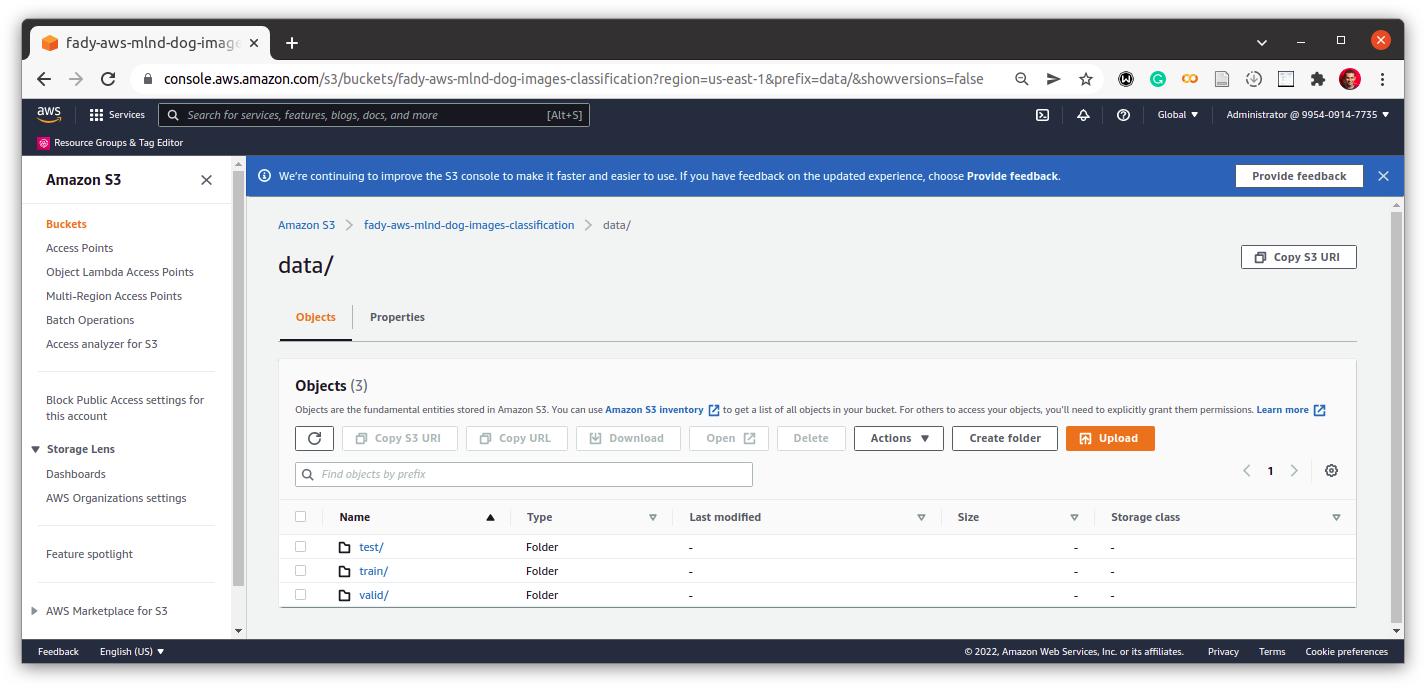
\includegraphics{../screenshots/01-b_s3-bucket.png}
\caption{S3 bucket}
\end{figure}

\newpage
\hypertarget{training-and-deployment-single-instance-training}{%
\subsection{Training and Deployment (Single Instance
Training)}\label{training-and-deployment-single-instance-training}}

From the fourth to the sixteenth cell of the
\href{https://github.com/FadyMorris/udacity-AWS-ml-engineer-nanodegree/tree/main/projects/04_operationalizing-an-aws-ml-project/train_and_deploy-solution.ipynb}{\texttt{train\_and\_deploy-solution.ipynb}}
notebook, I created a tuning job with an instance
type \texttt{ml.m5.xlarge}, \texttt{max\_jobs=2} and
\texttt{max\_parallel\_jobs=1} it took approximately 41 minutes to
complete. The best hyperparameters found were
\texttt{\{\textquotesingle{}batch\_size\textquotesingle{}:\ 32,\ \textquotesingle{}learning\_rate\textquotesingle{}:\ \textquotesingle{}0.00834462420525608\textquotesingle{}\}}

Then, I performed actual model training on the best hyperparameters
found by the tuner. This time I used \texttt{ml.m5.2xlarge} instance as
it has more processing power.

Then, I ran cells in the \textbf{Deployment} section of the notebook to
run an endpoint. I chose \texttt{ml.t2.medium} as it was sufficent for
the current inference task and I can run it for long hours to complete
the next steps of the projects and test lambda functions without
incurring too much charges.

Then, I tested it using the supplied request dict

\texttt{\{"url": "\url{https://s3.amazonaws.com/cdn-origin-etr.akc.org/wp-content/uploads/2017/11/20113314/Carolina-Dog-standing-outdoors.jpg}"\}}

and I got the following ineference vector:

\begin{Shaded}
\begin{Highlighting}[]
      \OtherTok{[} \FloatTok{0.13380046}\OtherTok{,}  \FloatTok{0.12406865}\OtherTok{,}  \FloatTok{0.01930925}\OtherTok{,}  \FloatTok{0.04459066}\OtherTok{,}  \FloatTok{0.31491399}\OtherTok{,}
        \FloatTok{0.14133964}\OtherTok{,} \FloatTok{{-}0.06225839}\OtherTok{,}  \FloatTok{0.15845889}\OtherTok{,} \FloatTok{{-}0.15713356}\OtherTok{,} \FloatTok{{-}0.06818745}\OtherTok{,}
        \FloatTok{0.12937857}\OtherTok{,}  \FloatTok{0.147229}  \OtherTok{,} \FloatTok{{-}0.06525478}\OtherTok{,}  \FloatTok{0.12964083}\OtherTok{,}  \FloatTok{0.19601114}\OtherTok{,}
        \FloatTok{0.07686417}\OtherTok{,}  \FloatTok{0.09087689}\OtherTok{,} \FloatTok{{-}0.02894698}\OtherTok{,} \FloatTok{{-}0.01715944}\OtherTok{,}  \FloatTok{0.16697152}\OtherTok{,}
        \FloatTok{0.1283621} \OtherTok{,} \FloatTok{{-}0.01064654}\OtherTok{,}  \FloatTok{0.10620853}\OtherTok{,}  \FloatTok{0.17278288}\OtherTok{,} \FloatTok{{-}0.03866604}\OtherTok{,}
       \FloatTok{{-}0.15799397}\OtherTok{,}  \FloatTok{0.14493701}\OtherTok{,} \FloatTok{{-}0.18795769}\OtherTok{,}  \FloatTok{0.27061909}\OtherTok{,}  \FloatTok{0.05165472}\OtherTok{,}
        \FloatTok{0.07323486}\OtherTok{,}  \FloatTok{0.11265536}\OtherTok{,} \FloatTok{{-}0.07641914}\OtherTok{,}  \FloatTok{0.14794479}\OtherTok{,}  \FloatTok{0.01756929}\OtherTok{,}
        \FloatTok{0.13642494}\OtherTok{,} \FloatTok{{-}0.03507356}\OtherTok{,}  \FloatTok{0.11343399}\OtherTok{,}  \FloatTok{0.1752239} \OtherTok{,}  \FloatTok{0.06675729}\OtherTok{,}
        \FloatTok{0.21560508}\OtherTok{,}  \FloatTok{0.11155353}\OtherTok{,}  \FloatTok{0.01593112}\OtherTok{,}  \FloatTok{0.14728004}\OtherTok{,}  \FloatTok{0.01010097}\OtherTok{,}
        \FloatTok{0.19000889}\OtherTok{,}  \FloatTok{0.01708234}\OtherTok{,}  \FloatTok{0.07144631}\OtherTok{,} \FloatTok{{-}0.0570593} \OtherTok{,} \FloatTok{{-}0.04598607}\OtherTok{,}
        \FloatTok{0.08687741}\OtherTok{,}  \FloatTok{0.00667302}\OtherTok{,} \FloatTok{{-}0.09806156}\OtherTok{,}  \FloatTok{0.07812651}\OtherTok{,}  \FloatTok{0.01943411}\OtherTok{,}
        \FloatTok{0.11979307}\OtherTok{,}  \FloatTok{0.12735154}\OtherTok{,} \FloatTok{{-}0.01926402}\OtherTok{,} \FloatTok{{-}0.07421727}\OtherTok{,}  \FloatTok{0.08052468}\OtherTok{,}
        \FloatTok{0.08618335}\OtherTok{,}  \FloatTok{0.05832509}\OtherTok{,}  \FloatTok{0.04668785}\OtherTok{,} \FloatTok{{-}0.14725739}\OtherTok{,} \FloatTok{{-}0.10800982}\OtherTok{,}
       \FloatTok{{-}0.22411092}\OtherTok{,} \FloatTok{{-}0.23320678}\OtherTok{,}  \FloatTok{0.14338717}\OtherTok{,}  \FloatTok{0.03731703}\OtherTok{,} \FloatTok{{-}0.01098941}\OtherTok{,}
        \FloatTok{0.16383903}\OtherTok{,} \FloatTok{{-}0.1022775} \OtherTok{,} \FloatTok{{-}0.10918213}\OtherTok{,} \FloatTok{{-}0.17303845}\OtherTok{,} \FloatTok{{-}0.11920816}\OtherTok{,}
        \FloatTok{0.08246608}\OtherTok{,} \FloatTok{{-}0.10248563}\OtherTok{,} \FloatTok{{-}0.12475339}\OtherTok{,}  \FloatTok{0.07674296}\OtherTok{,} \FloatTok{{-}0.03876449}\OtherTok{,}
        \FloatTok{0.0273919} \OtherTok{,}  \FloatTok{0.09122247}\OtherTok{,} \FloatTok{{-}0.06179177}\OtherTok{,} \FloatTok{{-}0.01053959}\OtherTok{,} \FloatTok{{-}0.19576041}\OtherTok{,}
        \FloatTok{0.0418855} \OtherTok{,}  \FloatTok{0.15541904}\OtherTok{,}  \FloatTok{0.02792337}\OtherTok{,}  \FloatTok{0.01690321}\OtherTok{,}  \FloatTok{0.06227571}\OtherTok{,}
        \FloatTok{0.0740654} \OtherTok{,} \FloatTok{{-}0.05714193}\OtherTok{,} \FloatTok{{-}0.21430534}\OtherTok{,} \FloatTok{{-}0.12310754}\OtherTok{,} \FloatTok{{-}0.09441458}\OtherTok{,}
       \FloatTok{{-}0.09090099}\OtherTok{,} \FloatTok{{-}0.02984259}\OtherTok{,} \FloatTok{{-}0.01214801}\OtherTok{,} \FloatTok{{-}0.09557887}\OtherTok{,} \FloatTok{{-}0.21917576}\OtherTok{,}
       \FloatTok{{-}0.08656652}\OtherTok{,} \FloatTok{{-}0.29427898}\OtherTok{,}  \FloatTok{0.05461352}\OtherTok{,} \FloatTok{{-}0.11696375}\OtherTok{,} \FloatTok{{-}0.25783783}\OtherTok{,}
       \FloatTok{{-}0.00612676}\OtherTok{,} \FloatTok{{-}0.02330022}\OtherTok{,} \FloatTok{{-}0.40888697}\OtherTok{,} \FloatTok{{-}0.08250632}\OtherTok{,} \FloatTok{{-}0.23096839}\OtherTok{,}
       \FloatTok{{-}0.0869923} \OtherTok{,}  \FloatTok{0.06188012}\OtherTok{,} \FloatTok{{-}0.14508837}\OtherTok{,} \FloatTok{{-}0.21565518}\OtherTok{,}  \FloatTok{0.07465033}\OtherTok{,}
       \FloatTok{{-}0.30452806}\OtherTok{,} \FloatTok{{-}0.04589951}\OtherTok{,}  \FloatTok{0.03223781}\OtherTok{,} \FloatTok{{-}0.31530797}\OtherTok{,} \FloatTok{{-}0.15733883}\OtherTok{,}
       \FloatTok{{-}0.37445912}\OtherTok{,} \FloatTok{{-}0.14996621}\OtherTok{,} \FloatTok{{-}0.07589076}\OtherTok{,}  \FloatTok{0.04984585}\OtherTok{,} \FloatTok{{-}0.25771111}\OtherTok{,}
       \FloatTok{{-}0.28103814}\OtherTok{,} \FloatTok{{-}0.13811049}\OtherTok{,} \FloatTok{{-}0.26339793}\OtherTok{,} \FloatTok{{-}0.03755928}\OtherTok{,} \FloatTok{{-}0.11867087}\OtherTok{,}
       \FloatTok{{-}0.28322217}\OtherTok{,} \FloatTok{{-}0.40221205}\OtherTok{,} \FloatTok{{-}0.3020235} \OtherTok{]}
\end{Highlighting}
\end{Shaded}

\newpage
The endpint name is
\texttt{\textquotesingle{}pytorch-inference-2022-01-20-04-04-06-315\textquotesingle{}}
and is shown in the following screenshot:

\begin{figure}[H]
\centering
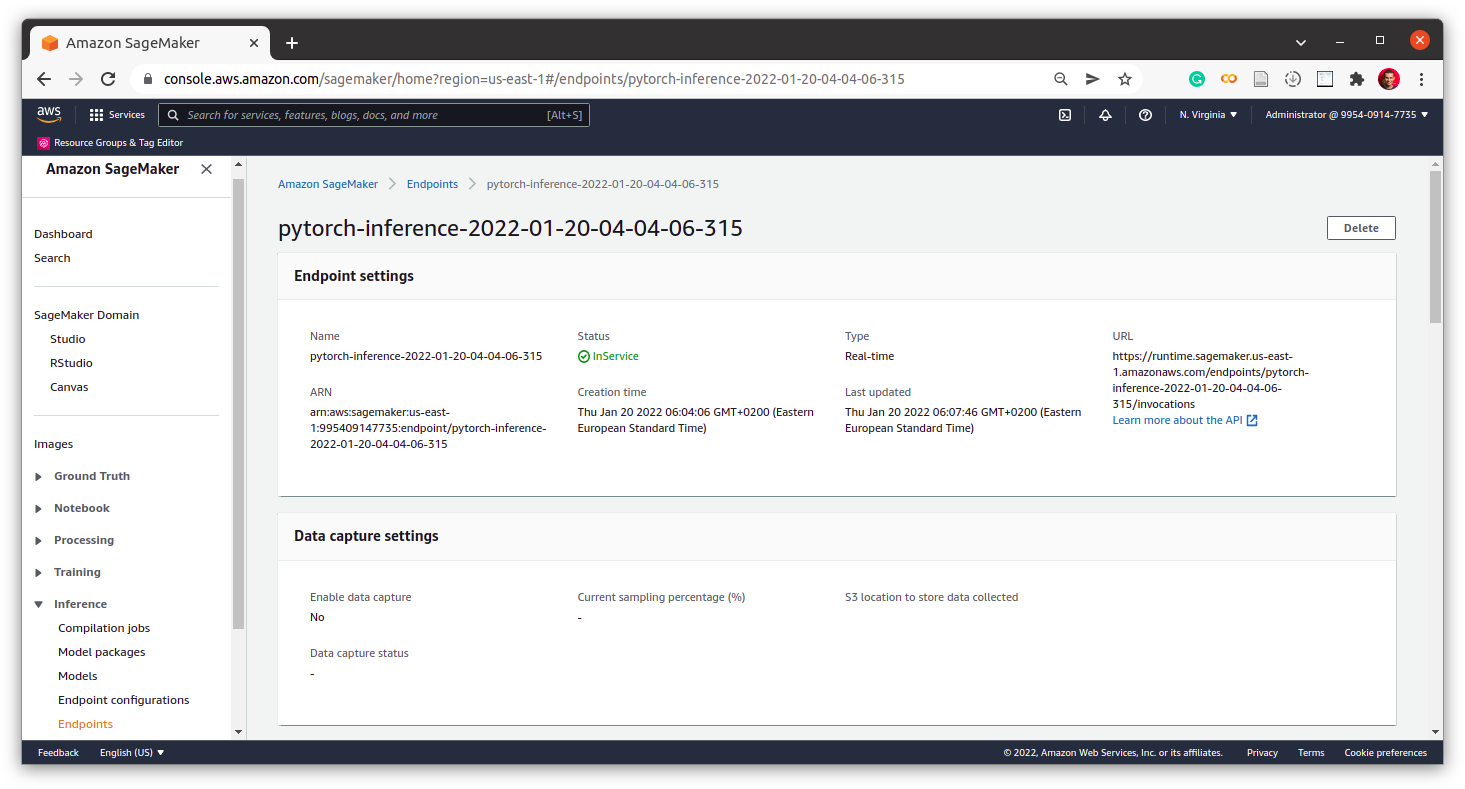
\includegraphics[width=0.95\textwidth]{../screenshots/01-c_endpoint-1_single-instance-training.png}
%\caption{Endpoint - Single Instance}
\end{figure}

\hypertarget{training-and-deployment-multi-instance-training}{%
\section{Training and Deployment (Multi-instance
training)}\label{training-and-deployment-multi-instance-training}}

I created a multi-instance training job by modifying the parameter
\texttt{insance\_count=4} to run 4 instances simultanously for training.

\begin{lstlisting}[language=Python]
estimator_multi_instance = PyTorch(
  ... ,
  instance_count = 4,
  ...
)
\end{lstlisting}


Then I deployed another endpoint, the endpint name is
\texttt{\textquotesingle{}pytorch-inference-2022-01-20-04-28-29-950\textquotesingle{}}
and is shown in the following screenshot:

\begin{figure}[H]
\centering
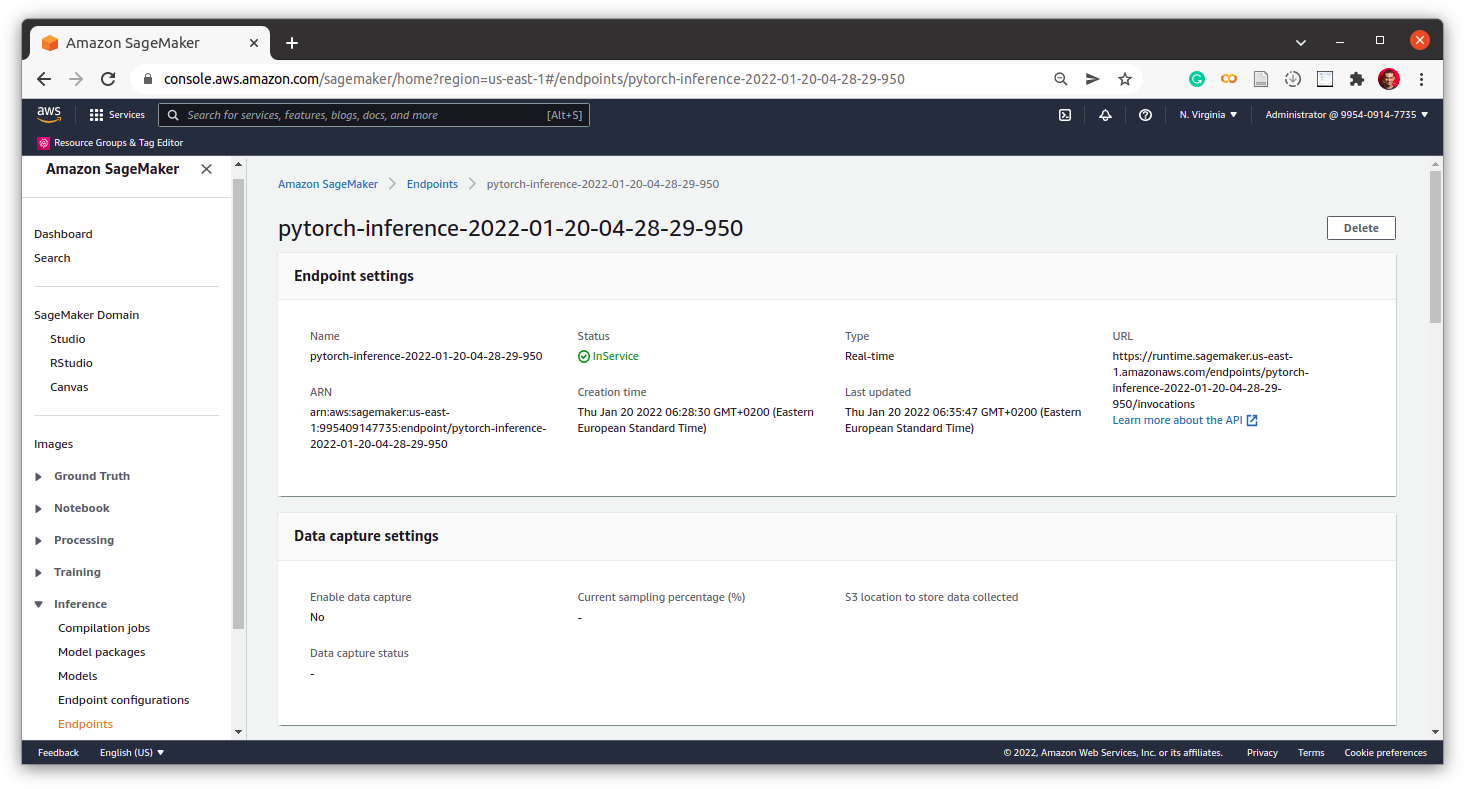
\includegraphics[width=0.95\textwidth]{../screenshots/01-c_endpoint-2_multi-instance-training.png}
%\caption{Endpoint - Multi-instance}
\end{figure}

\hypertarget{step-2-ec2-training}{%
\section{Step 2: EC2 Training}\label{step-2-ec2-training}}

I used
\href{https://aws.amazon.com/ec2/instance-types/m5/}{\texttt{m5.2xlarge}}.
I ran multiple experiments in
\href{https://github.com/FadyMorris/udacity-AWS-ml-engineer-nanodegree/tree/main/projects/03_image-classification-aws-sagemaker}{Project 03 -
image-classification-aws-sagemaker} with training 1 epoch of the dataset
and I found out that this instance has a decent value per dollar. The
results can be shown in the following table:

\begin{longtable}[]{@{}
  >{\raggedright\arraybackslash}p{(\columnwidth - 14\tabcolsep) * \real{0.12}}
  >{\raggedleft\arraybackslash}p{(\columnwidth - 14\tabcolsep) * \real{0.10}}
  >{\raggedleft\arraybackslash}p{(\columnwidth - 14\tabcolsep) * \real{0.08}}
  >{\raggedleft\arraybackslash}p{(\columnwidth - 14\tabcolsep) * \real{0.18}}
  >{\raggedleft\arraybackslash}p{(\columnwidth - 14\tabcolsep) * \real{0.17}}
  >{\raggedleft\arraybackslash}p{(\columnwidth - 14\tabcolsep) * \real{0.12}}
  >{\raggedleft\arraybackslash}p{(\columnwidth - 14\tabcolsep) * \real{0.14}}
  >{\raggedleft\arraybackslash}p{(\columnwidth - 14\tabcolsep) * \real{0.09}}@{}}
\toprule
\begin{minipage}[b]{\linewidth}\raggedright
compute instance
\end{minipage} & \begin{minipage}[b]{\linewidth}\raggedleft
billing time
\end{minipage} & \begin{minipage}[b]{\linewidth}\raggedleft
cost/hour
\end{minipage} & \begin{minipage}[b]{\linewidth}\raggedleft
Epoch training time(sec)
\end{minipage} & \begin{minipage}[b]{\linewidth}\raggedleft
Epoch testing time(sec)
\end{minipage} & \begin{minipage}[b]{\linewidth}\raggedleft
setup time(sec)
\end{minipage} & \begin{minipage}[b]{\linewidth}\raggedleft
training cost/epoch
\end{minipage} & \begin{minipage}[b]{\linewidth}\raggedleft
total cost
\end{minipage} \\
\midrule
\endhead
ml.m5.large & 1980 & 0.115 & 1648.37 & 156.01 & 175.62 & 0.053 &
0.063 \\
ml.m5.xlarge & 1164 & 0.23 & 894.19 & 92.23 & 177.58 & 0.057 & 0.074 \\
ml.p2.xlarge & 601 & 1.125 & 163.52 & 16.18 & 421.3 & 0.051 & 0.188 \\
ml.m5.4xlarge & 538 & 0.922 & 336.38 & 46.23 & 155.39 & 0.086 & 0.138 \\
ml.c4.4xlarge & 648 & 0.955 & 398.55 & 52.32 & 197.13 & 0.106 & 0.172 \\
ml.m5.2xlarge & 742 & 0.461 & 518.4 & 60.69 & 162.91 & 0.066 & 0.095 \\
ml.g4dn.12xlarge & 473 & 4.89 & 111.42 & 9.67 & 351.91 & 0.151 &
0.642 \\
ml.p3.2xlarge & 495 & 3.825 & 108.59 & 11.17 & 375.24 & 0.115 & 0.526 \\
\bottomrule
\end{longtable}

As a training image, I used
\href{https://console.aws.amazon.com/ec2/v2/home?region=us-east-1\#ImageDetails:imageId=ami-06ada98f5d02a2d2d}{\texttt{Deep\ Learning\ AMI\ (Amazon\ Linux\ 2)\ Version\ 57.0\ -\ ami-06ada98f5d02a2d2d}}
to train the model.

The command that is used to create the instance with the deep learning
image is:

\begin{lstlisting}[language=sh]
  aws ec2 run-instances --image-id ami-06ada98f5d02a2d2d --count 1 --instance-type m5.2xlarge --key-name <kms-key-name> --security-groups <security-group-name>
\end{lstlisting}


Screenshot of the created instance:

\begin{figure}[H]
\centering
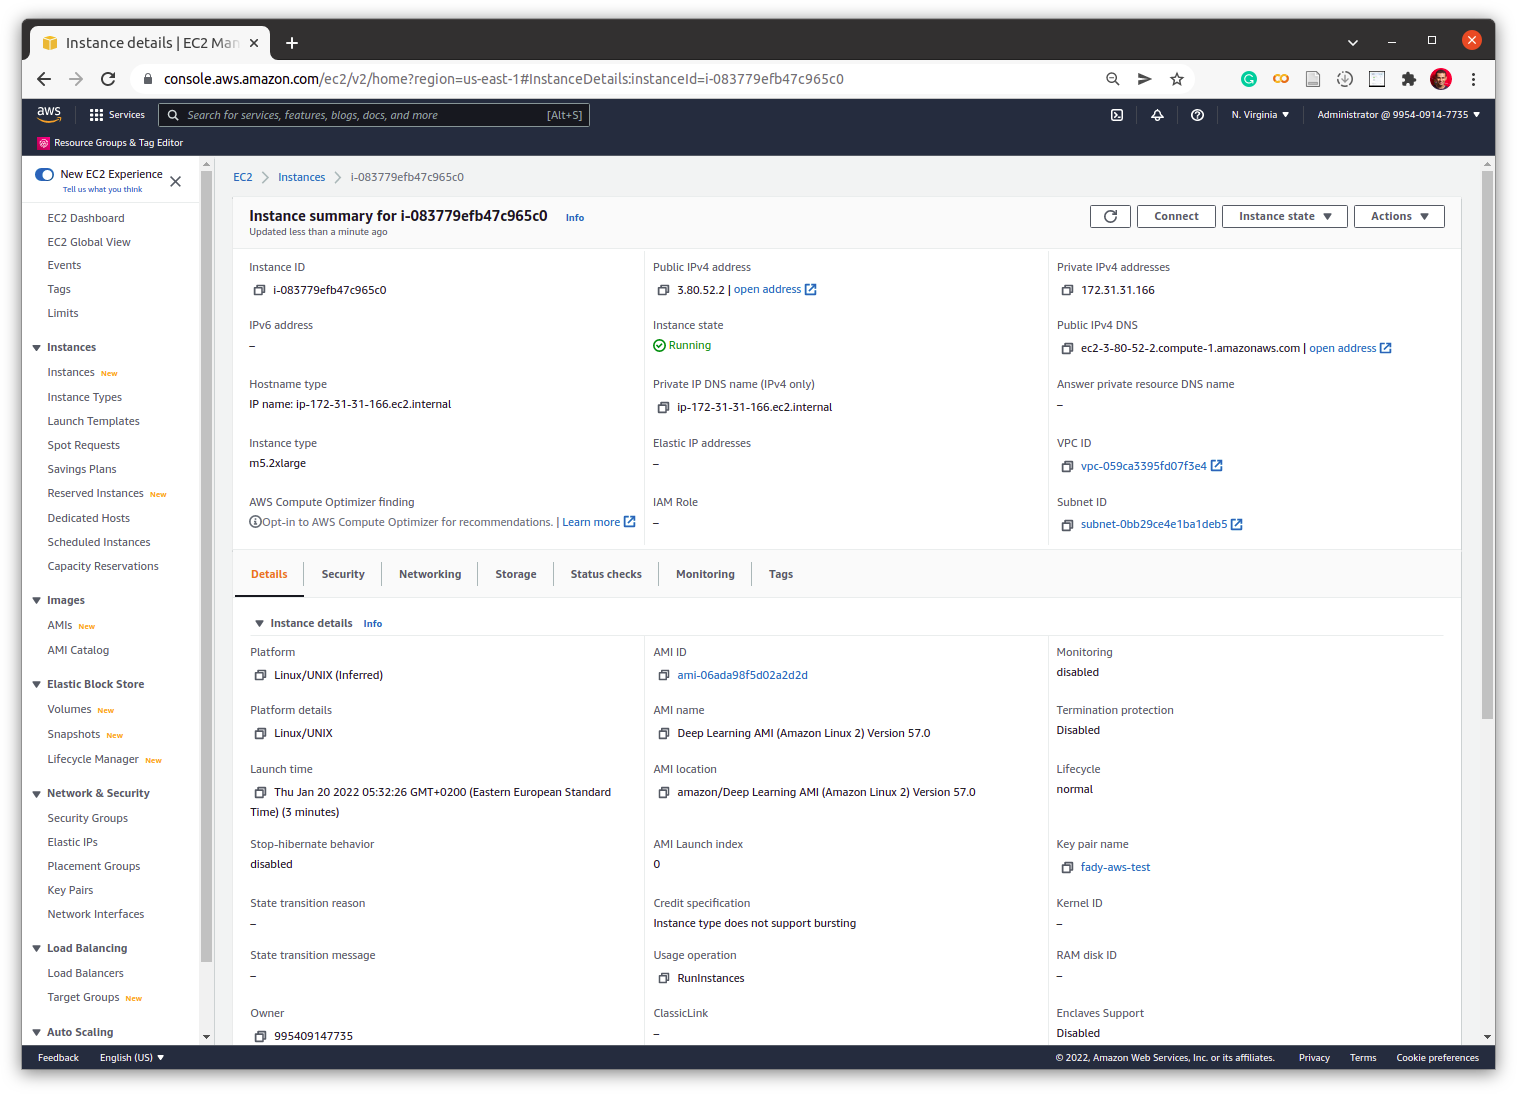
\includegraphics{../screenshots/02-a_ec2-instance.png}
\caption{EC2 Instance}
\end{figure}

Then I used ssh to connect to the instance:

\begin{lstlisting}[language=bash]
ssh -i "fady-aws-test.pem" ec2-user@ec2-3-80-52-2.compute-1.amazonaws.com
\end{lstlisting}

Download the data and create model output directory:

\begin{lstlisting}[language=bash]
wget https://s3-us-west-1.amazonaws.com/udacity-aind/dog-project/dogImages.zip
unzip dogImages.zip
mkdir TrainedModels
\end{lstlisting}


Paste the contents of \href{https://github.com/FadyMorris/udacity-AWS-ml-engineer-nanodegree/tree/main/projects/04_operationalizing-an-aws-ml-project/ec2train1.py}{ec2train1.py} inside \texttt{solution.py} on
the machine

\begin{lstlisting}[language=bash]
vim solution.py
\end{lstlisting}

Activate the \texttt{pytorch} environment that we will use to train our
model:

\begin{lstlisting}[language=bash]
conda activate aws_neuron_pytorch_p36
\end{lstlisting}


Train the model

\begin{lstlisting}[language=bash]
python solution.py
\end{lstlisting}

Screenshot of final model training step in terminal:

\begin{figure}[H]
\centering
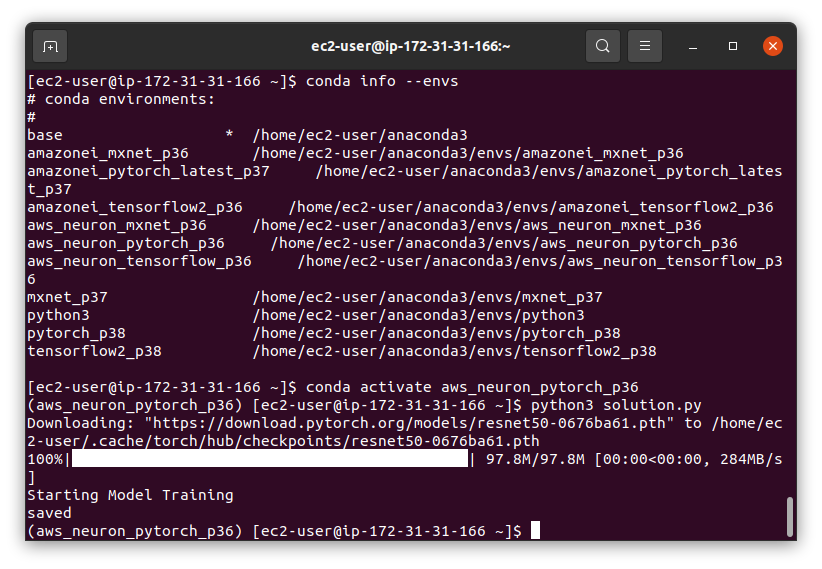
\includegraphics{../screenshots/02-b_ec2-terminal-ssh.png}
\caption{EC2 Terminal}
\end{figure}

\newpage
\hypertarget{difference-between-ec2-training-code-and-the-code-used-in-sagemaker}{%
\subsection{Difference Between EC2 Training Code and the Code used in
Sagemaker}\label{difference-between-ec2-training-code-and-the-code-used-in-sagemaker}}

For EC2 Training we executed \href{https://github.com/FadyMorris/udacity-AWS-ml-engineer-nanodegree/tree/main/projects/04_operationalizing-an-aws-ml-project/ec2train1.py}{\texttt{ec2train1.py}}
directly inside the instance. While in Sagemaker we executed deployment
code from cells in \url{train_and_deploy-solution.ipynb} that created a
new training job instance and copied the training script
\href{https://github.com/FadyMorris/udacity-AWS-ml-engineer-nanodegree/tree/main/projects/04_operationalizing-an-aws-ml-project/hpo.py}{\texttt{hpo.py}} to it to do the training.

\textbf{Major differences:}

\begin{itemize}
\tightlist

\item Executing
\href{https://github.com/FadyMorris/udacity-AWS-ml-engineer-nanodegree/tree/main/projects/04_operationalizing-an-aws-ml-project/ec2train1.py}{\texttt{ec2train1.py}} directly from the command
line performs the training locally on the same compute machine. While in
the Sagemaker notebook \url{train_and_deploy-solution.ipynb} it spawns
another compute instance and pass all the training parameters to it.

\item The hyperparameters in Sagemaker starter script
\href{https://github.com/FadyMorris/udacity-AWS-ml-engineer-nanodegree/tree/main/projects/04_operationalizing-an-aws-ml-project/hpo.py}{\texttt{hpo.py}} are passed explicitly to the script and
recorded in the instance environment variables.

\href{https://github.com/FadyMorris/udacity-AWS-ml-engineer-nanodegree/tree/main/projects/04_operationalizing-an-aws-ml-project/hpo.py}{\texttt{hpo.py}} execution command:

\begin{lstlisting}[]
/opt/conda/bin/python3.6 hpo.py --batch_size 32 --learning_rate 0.00834462420525608
\end{lstlisting}

\href{https://github.com/FadyMorris/udacity-AWS-ml-engineer-nanodegree/tree/main/projects/04_operationalizing-an-aws-ml-project/hpo.py}{\texttt{hpo.py}} argument parsing:

\begin{lstlisting}[language=Python]
parser.add_argument('--learning_rate', type=float)
parser.add_argument('--batch_size', type=int)
parser.add_argument('--data', type=str, default=os.environ['SM_CHANNEL_TRAINING'])
parser.add_argument('--model_dir', type=str, default=os.environ['SM_MODEL_DIR'])
parser.add_argument('--output_dir', type=str, default=os.environ['SM_OUTPUT_DATA_DIR'])
\end{lstlisting}

Instance environment variables:

\begin{lstlisting}
SM_USER_ARGS=["--batch_size","32","--learning_rate","0.00834462420525608"]
SM_HPS={"batch_size":32,"learning_rate":"0.00834462420525608"}
SM_HP_BATCH_SIZE=32
SM_HP_LEARNING_RATE=0.00834462420525608
SM_CHANNEL_TRAINING=/opt/ml/input/data/training
SM_MODEL_DIR=/opt/ml/model
SM_OUTPUT_DIR=/opt/ml/output
SM_USER_ENTRY_POINT=hpo.py
\end{lstlisting}

In \href{https://github.com/FadyMorris/udacity-AWS-ml-engineer-nanodegree/tree/main/projects/04_operationalizing-an-aws-ml-project/ec2train1.py}{\texttt{ec2train1.py}}, the hyperparameters are
included in the script.

\begin{lstlisting}[language=Python]
batch_size=2
learning_rate=1e-4
\end{lstlisting}

\href{https://github.com/FadyMorris/udacity-AWS-ml-engineer-nanodegree/tree/main/projects/04_operationalizing-an-aws-ml-project/ec2train1.py}{\texttt{ec2train1.py}} execution command:

\begin{lstlisting}[language=bash]
python ec2train1.py
\end{lstlisting}

\item
  In Sagemaker, the output trained model \texttt{model.pth} is saved to
  the training job compute instance \linebreak
  \texttt{SM\_MODEL\_DIR=/opt/ml/model} , then it is compressed with the
  source code \href{https://github.com/FadyMorris/udacity-AWS-ml-engineer-nanodegree/tree/main/projects/04_operationalizing-an-aws-ml-project/hpo.py}{\texttt{hpo.py}} and the model artifact is
  transferred automatically to an output directory in the S3 bucket.
  While in EC2 training the model is saved locally inside
  \texttt{./TrainedModels} and the user is responsible of saving the
  model to S3 using \colorbox{gray!10}{\lstinline{aws s3 cp}} command.
\item
  Sagemaker can use the training script to spawn multiple instances and
  perform distributed training. While EC2 instance is just limited to
  the one instance that the script is run on.
\end{itemize}

\hypertarget{step-3-setting-up-a-lambda-function}{%
\section{Step 3: Setting up a Lambda
function}\label{step-3-setting-up-a-lambda-function}}

The supplied lambda function
\href{https://github.com/FadyMorris/udacity-AWS-ml-engineer-nanodegree/tree/main/projects/04_operationalizing-an-aws-ml-project/lamdafunction.py}{\texttt{lamdafunction.py}} was patched with the
deployed endpoint that we created in previous steps
\texttt{endpoint\_Name=\textquotesingle{}pytorch-inference-2022-01-20-04-28-29-950\textquotesingle{}}

The function only accepts image URL passed as a request dictionary with
content type \texttt{application/json}. The request dictionary has the
format
\texttt{\{\textquotesingle{}url\textquotesingle{}:\textquotesingle{}http://website.com/image-url.ext\textquotesingle{}\}}

It invokes the \texttt{pytorch-inference-2022-01-20-04-28-29-950}
endpoint, passing the request dictionary
(\texttt{\{\textquotesingle{}url\textquotesingle{}:\ \textquotesingle{}http://....\textquotesingle{}\}})
in the body and setting the content type to \texttt{application/json}.
The endpoint returns the predictions to the lambda function and the
lambda function returns the predictions to the user in the body of the
response, with a status code 200.

\newpage
\hypertarget{step-4-lambda-security-and-testing}{%
\section{Step 4: Lambda Security and
Testing}\label{step-4-lambda-security-and-testing}}

In this step we created an IAM execution role
\texttt{arn:aws:iam::995409147735:role/fady-project-4-lambda-execution-role}
for our lambda function and attached
\href{https://console.aws.amazon.com/iam/home\#/policies/arn:aws:iam::aws:policy/AmazonSageMakerFullAccess}{\texttt{AmazonSageMakerFullAccess}}
security policy to it.

\hypertarget{lambda-function-testing}{%
\subsection{Lambda function testing}\label{lambda-function-testing}}

I tested the lambda function on the following dog image:

\begin{figure}[H]
  \centering
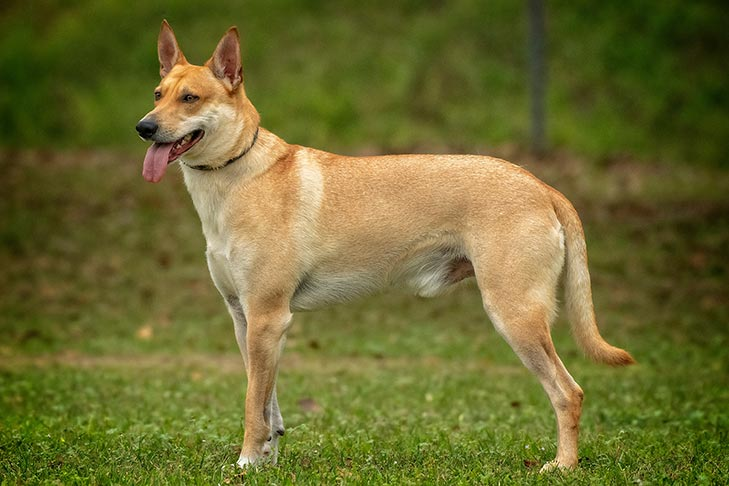
\includegraphics[width=0.75\linewidth]{../Carolina-Dog-standing-outdoors.jpg}
%\caption{Carolina Dog Standing Outdoors}
\end{figure}

using the supplied request dict


\texttt{\{"url": "\url{https://s3.amazonaws.com/cdn-origin-etr.akc.org/wp-content/uploads/2017/11/20113314/Carolina-Dog-standing-outdoors.jpg}"\}}


the result is shown in the following screenshot:

\begin{figure}[H]
\centering
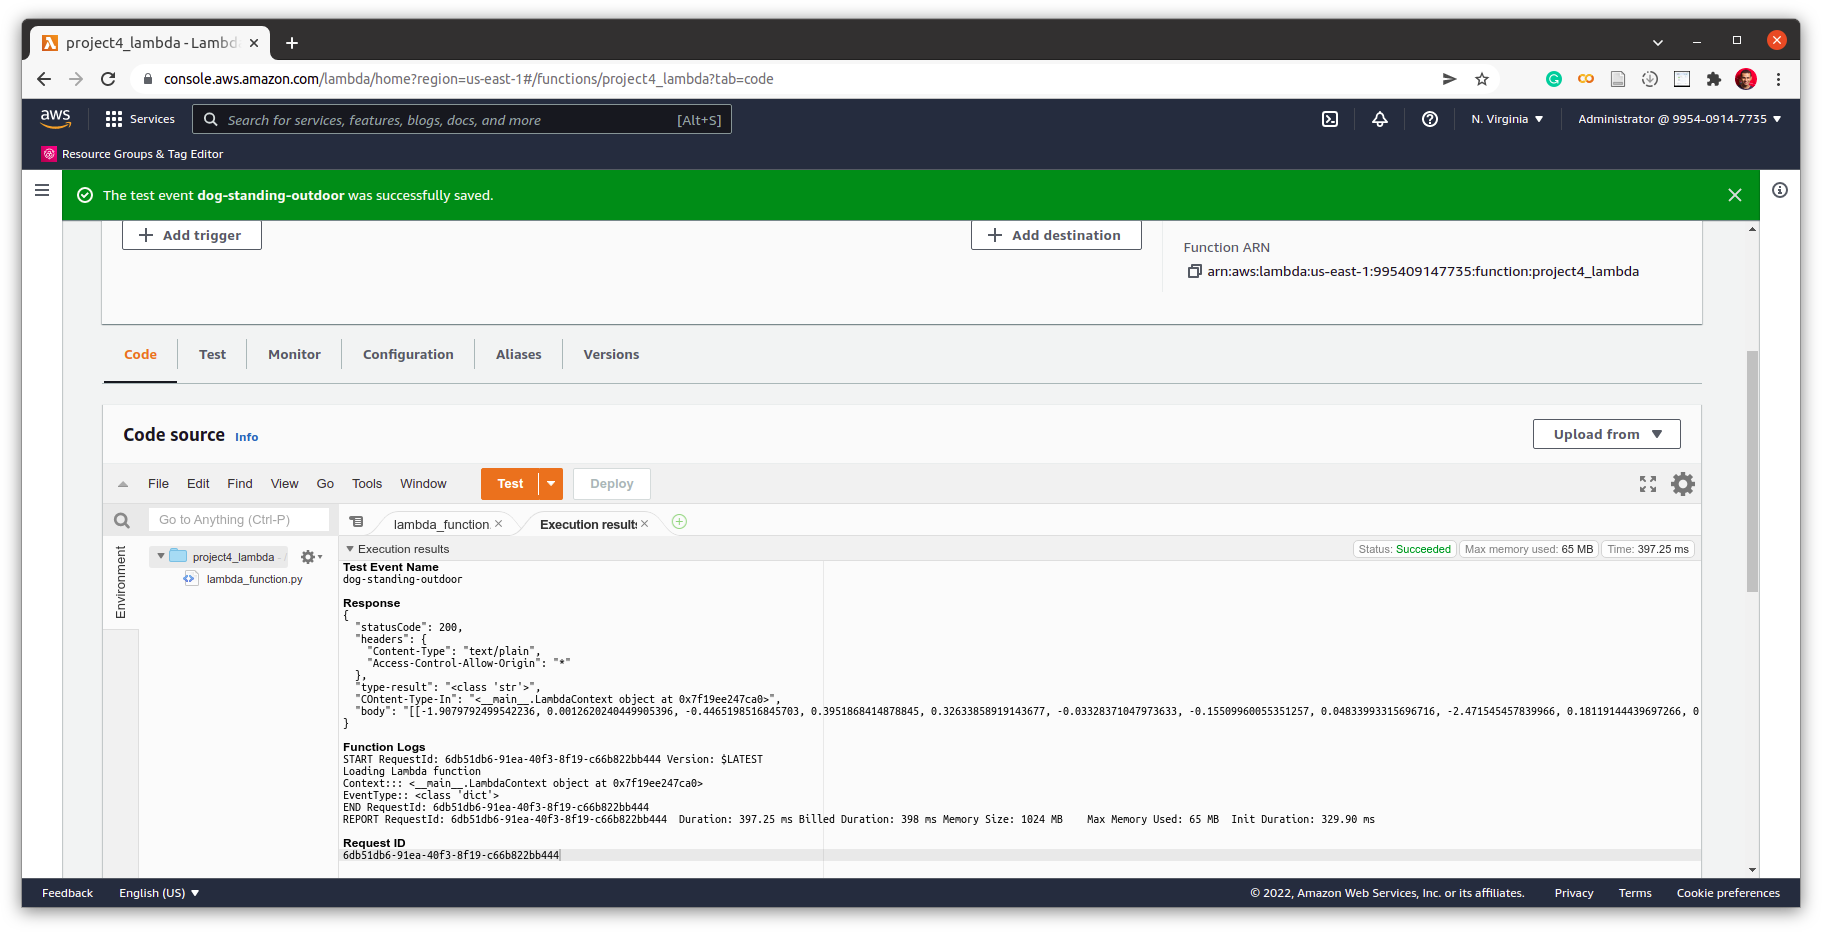
\includegraphics{../screenshots/04-a_lambda-function-testing.png}
%\caption{Lambda function successful test}
\end{figure}

\hypertarget{security-considerations}{%
\subsection{Security considerations}\label{security-considerations}}

The
\href{https://console.aws.amazon.com/iam/home\#/policies/arn:aws:iam::aws:policy/AmazonSageMakerFullAccess}{\texttt{AmazonSageMakerFullAccess}}
policy may be too much for our lambda function that only executes
endpoints from sagemaker. Perhaps restricting it to endpoints only would
be a better practice.

Also care should be taken to delete unused lambdas and roles and give
the least priviliges to resources in use to pervent vulnerabilities.

Screenshot of the IAM role used to execute the lambda function:

\begin{figure}[H]
\centering
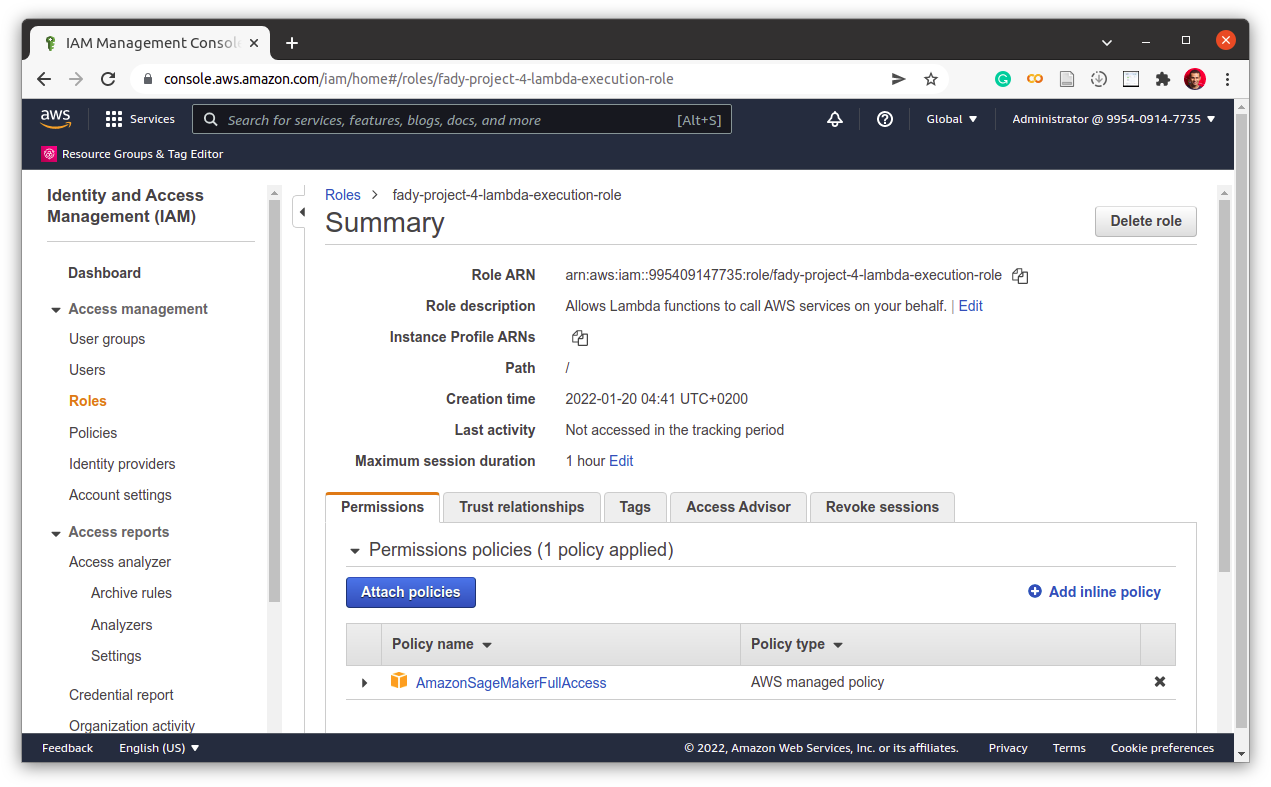
\includegraphics{../screenshots/04-b_IAM-role.png}
\caption{IAM role}
\end{figure}

\newpage

\hypertarget{step-5-concurrency-and-auto-scaling}{%
\section{Step 5: Concurrency and
auto-scaling}\label{step-5-concurrency-and-auto-scaling}}

\hypertarget{concurrency}{%
\subsection{Concurrency}\label{concurrency}}

oncurrency refers to the ability of Lambda functions to service multiple
requests at once

We can use either reserved or provisioned concurrency for our function.
Provisioned concurrency is more responsive, but leads to higher costs.

Since we don't expect very high volumes on these functions, it's not
necessary to choose very high concurrency. I set the provisioned
concurrency to 3 and it is enough for our load, and 100 for reserved
concurrency.

Screenshot of lambda concurrency settings:

\begin{figure}[H]
\centering
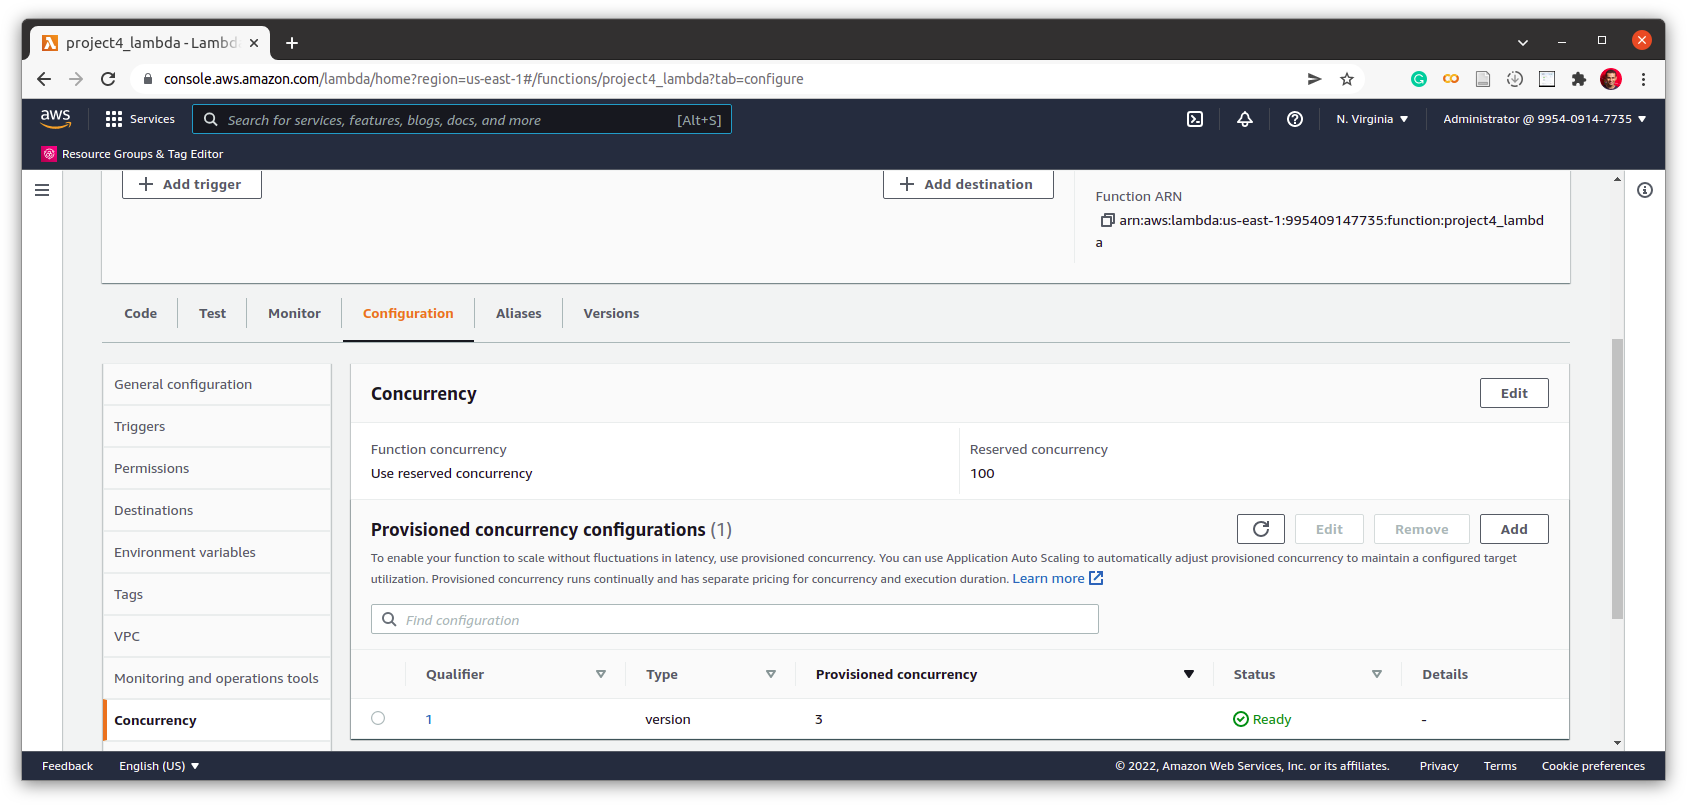
\includegraphics{../screenshots/05_lambda-concurrency.png}
\caption{Lambda function concurrency settings}
\end{figure}

\hypertarget{auto-scaling}{%
\subsection{Auto-scaling}\label{auto-scaling}}

Auto-scaling refers to the ability of endpoints to service multiple
lambda function requests at once. I chose to autoscale endpoints to 4
instances maximum, with scale in coold down time of 30 seconds and scale
out cool down time of 300 seconds. These settings are sufficient for our
project needs and workload.

\end{document}

%%% Local Variables:
%%% mode: latex
%%% TeX-engine: xetex
%%% TeX-master: t
%%% End:
